\documentclass[border={5pt 5pt 5pt 5pt}]{standalone}
\usepackage[american]{circuitikz}

\begin{document}

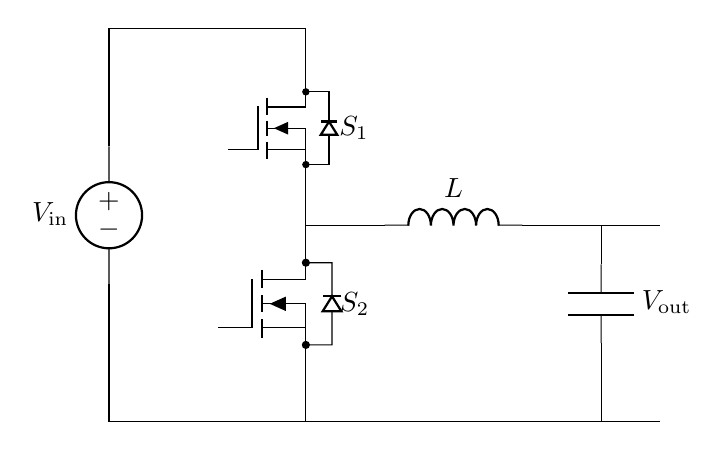
\begin{tikzpicture}
	% Paths, nodes and wires:
	\draw (4.5, 9.5) to[american voltage source, l_={$V_{\mathrm{in}}$}] (4.5, 7.75);
	\draw (7, 9) -| (7, 8.25);
	\draw (8, 8.5) to[american inductor, l={$L$}] (9.75, 8.5);
	\draw (10.75, 8) to[capacitor, l={$V_{\mathrm{out}}$}] (10.75, 7);
	\draw (8, 8.5) -- (7, 8.5);
	\draw (9.75, 8.5) -- (11.5, 8.5);
	\draw (10.75, 8) -| (10.75, 8.5);
	\draw (10.75, 7) -| (10.75, 6);
	\draw (7, 6) -- (11.5, 6);
	\node[nigfete, bodydiode](N1) at (7, 9.73){} node[anchor=west] at ([xshift=0.23cm]N1.text){$S_1$};
	\node[nigfete, bodydiode, xscale=1.13, yscale=1.13](N2) at (7, 7.5){} node[anchor=west] at ([xshift=0.23cm]N2.text){$S_2$};
	\draw (4.5, 7.75) -- (4.5, 6) -- (7, 6);
	\draw (7, 6.73) -| (7, 6);
	\draw (4.5, 9.5) -| (4.5, 11);
	\draw (4.5, 11) -- (7, 11);
	\draw (7, 11) -| (7, 10.5);
\end{tikzpicture}

\end{document}
